\documentclass[twocolumn,twoside,a4paper, 10pt]{IEEEtran}

\usepackage[utf8]{inputenc}
\usepackage[T1]{fontenc}
\usepackage[noadjust]{cite}
\renewcommand{\citepunct}{,\penalty\citepunctpenalty\,}
\renewcommand{\citedash}{--}
\usepackage{lipsum}

%\usepackage[catalan]{babel} %Idioma Català
%\usepackage[spanish]{babel}  %Idioma Castellano
\usepackage[english]{babel} %Language English

\usepackage{url}
\usepackage{graphicx}

% % % % % % % % % % % % % % % % % %
%     ACTUALIZA PARA TU CASO      %
% % % % % % % % % % % % % % % % % %
\title{Development of a Centralized Network Controller and mechanisms for its Duplication over Time-Sensitive Networking (TSN) Ethernet Networks}

\author{\normalsize 
{\large Andreu Marc Servera Lauder } \\
 \textbf{Tutor:}  {\large Inés Álvarez Vadillo, Julián Proenza Arenas} \\
Trabajo de fin de Máster Universitario en Sistemas Inteligentes (MUSI)\\
Universitat de les Illes Balears \\
07122 Palma, Illes Balears, Espanya \\
\url{andreumarc12@gmail.com}
}
% % % % % % % % % % % % % % % % % %

\begin{document}

\thispagestyle{empty}
%\onecolumn
\begin{center}

% % % % % % % % % % % % % % % % % % % % % % % %
%     ACTUALITZA EL CONTINGUT PEL TEU CAS     %
% % % % % % % % % % % % % % % % % % % % % % % %

\vspace*{1cm}

\includegraphics[scale=1]{figures/logo.png}

\vspace*{2.2cm}
\LARGE {\textbf{T\'itol}:} \\
\vspace*{1cm}

\noindent \Large{Autor: Nom i cognoms, i signatura\\}
\vspace*{1.5cm}

\noindent \large \textbf{Memòria del Treball de Fi de Màster} \\
\vspace*{0.5cm}
\noindent {M\`aster Universitari en Sistemes Intel·ligents (MUSI)
} \\
\noindent \large {de la} \\
\noindent \large {UNIVERSITAT DE LES ILLES BALEARS} \\
\vspace*{0.5cm}
\noindent \large {Curs Acadèmic 20xx-20xx} \\
\vspace*{1cm}

\vspace*{0.75cm}
\noindent \Large DD/MM/AAAA

\vspace*{1cm}
\noindent \large{Tutor: Nom i cognoms, i signatura\\}

%Descomenta pel tutor 2
%\vspace*{0.5cm}
%\noindent \large{Tutor: Nom i cognoms, i signatura\\}

%Descomenta pel tutor 3
%\vspace*{0.5cm}
%\noindent \large{Tutor: Nom i cognoms, i signatura\\}


\end{center}
\twocolumn
\newpage %Portada Català
%\onecolumn
\begin{center}

% % % % % % % % % % % % % % % % % % % % % % % %
%     ACTUALIZA EL CONTENIDO PARA TU CASO     %
% % % % % % % % % % % % % % % % % % % % % % % %

\vspace*{1cm}

\includegraphics[scale=1]{figures/logo.png}

\vspace*{2.2cm}
\LARGE {\textbf{T\'itulo}: Development of a Centralized Network Controller and mechanisms for its Duplication over Time-Sensitive Networking (TSN) Ethernet Networks} \\
\vspace*{1cm}

\noindent \Large{Autor: Nombre y apellidos, y firma\\}
\vspace*{1.5cm}

\noindent \large \textbf{Memoria del Trabajo de Fin de Máster} \\
\vspace*{0.5cm}
\noindent {M\'aster Universitario en Sistemas Inteligentes (MUSI)
} \\
\noindent \large {de la} \\
\noindent \large {UNIVERSITAT DE LES ILLES BALEARS} \\
\vspace*{0.5cm}
\noindent \large {Curso Académico 20xx-20xx} \\
\vspace*{1cm}

\vspace*{0.75cm}
\noindent \Large DD/MM/AAAA

\vspace*{1cm}
\noindent \large{Tutor: Nombre y apellidos, y firma\\}

%Descomenta pel tutor 2
%\vspace*{0.5cm}
%\noindent \large{Tutor: Nombre y apellidos, y firma\\}

%Descomenta pel tutor 3
%\vspace*{0.5cm}
%\noindent \large{Tutor: Nombre y apellidos, y firma\\}


\end{center}
\twocolumn
\newpage %Portada Castellà
\onecolumn
\begin{center}

% % % % % % % % % % % % % % % % % % % % % % % %
%     UPDATE THE CONTENTS IN YOUR CASE        %
% % % % % % % % % % % % % % % % % % % % % % % %

\vspace*{1cm}

\includegraphics[scale=1]{figures/logo.png}

\vspace*{2.2cm}
\LARGE {\textbf{Title}: Development of a Centralized Network Controller and mechanisms for its Duplication over Time-Sensitive Networking (TSN) Ethernet Networks.} \\
\vspace*{1cm}

\noindent \Large{Author: Andreu Marc Servera Lauder\\}
\vspace*{1.5cm}

\noindent \large \textbf{Master's Thesis} \\
\vspace*{0.5cm}
\noindent {Master's Degree in Intelligent Systems (MUSI)
} \\
\noindent \large {at the} \\
\noindent \large {UNIVERSITAT DE LES ILLES BALEARS} \\
\vspace*{0.5cm}
\noindent \large {Academic Year 2020-2021} \\
\vspace*{1cm}

\vspace*{0.75cm}
\noindent \Large DD/MM/YYYY

\vspace*{1cm}
\noindent \large{Supervisor: Julián Proenza Arenas\\}

%Uncomment for supervisor 2
\vspace*{0.5cm}
\noindent \large{Supervisor: Inés Álvarez Vadillo\\}

%Uncomment for supervisor 3
%\vspace*{0.5cm}
%\noindent \large{Supervisor: Name and surname, and signature\\}


\end{center}
\twocolumn
\newpage %Cover English
\maketitle
\thispagestyle{empty}


% % % % % % % % % % % % % % % % % %
%     ACTUALIZA PARA TU CASO      %
% % % % % % % % % % % % % % % % % %
\begin{abstract}
\noindent Plantilla de estilo para la redacción de la memoria del Trabajo de Fin de Máster del Máster Universitario en Sistemas Inteligentes (MUSI) basada en IEEEtran y adaptada por Ramon Mas y Sebastià Massanet, coordinadores del TFM.
\end{abstract}

\section*{Abstract}
\noindent  Template for the Master's Thesis for the Master's Degree in Intelligent Systems (MUSI) based on IEEEtran and adapted by Ramon Mas and Sebastià Massanet, coordinators of the Master's Thesis subject.\par
\noindent  \textit{El resumen en inglés es obligatorio.}


\begin{keywords}
One, two, three, four, five
\end{keywords}

\section{Motivación}

Estas normas son de obligado cumplimiento para todos los alumnos del trabajo de fin de máster.  No cumplir estas normas puede llevar a la no aceptación del trabajo. 

\section{Normas fundamentales \label{sec:fund}} 

\subsection{El cuerpo, la fuente y las líneas}

No se puede modificar el estilo del cuerpo, la fuente ni el estilo de línea. El cuerpo se divide en dos columnas. El texto es de fuente Times y de tamaño 10~puntos. El texto debe quedar justificado a ambos márgenes. En la última página las columnas deben quedar equilibradas. Un inicio de párrafo queda indicado porque la primera palabra está indentada.

\subsection{Figuras y cuadros}

Las figuras y los cuadros pueden ir dentro de una columna o dentro del cuerpo. En ambos casos la figura o el cuadro están centrados dentro de la columna o el cuerpo. Ambos entornos van numerados y tienen numeraciones independientes. El pie de figura empieza con \emph{Figura n:}, usa texto normal a 10~puntos y se sitúa debajo de la figura. En cambio, el pie de cuadro se situa en la parte superior del cuadro. En la figura \ref{fig:fig1}, se puede observar una figura situada dentro de la columna, mientras que la figura \ref{fig:fig2} representa un ejemplo de figura situada dentro del cuerpo. En el cuadro \ref{tab:table1}, se dispone de un ejemplo de cuadro que ocupa ambas columnas.

\begin{figure}
\begin{center}
	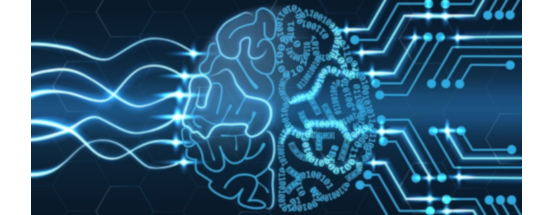
\includegraphics[width = \linewidth]{figures/logo-MUSI.png}
\end{center}
\caption{Figura dentro de la columna.} \label{fig:fig1}
\end{figure}

\begin{figure*}
\begin{center}
	
\includegraphics[width = \linewidth]{figures/fig2.png}
\end{center}
\caption{Figura dentro del cuerpo. Créditos phdcomics.} \label{fig:fig2}
\end{figure*}

Si el objeto está dentro de una columna puede ir en cualquier lugar de la misma, pero si ocupa ambas columnas sólo puede ir en la parte superior o inferior de la página.

\begin{table*}
	\caption{Algunas asignaturas del Máster MUSI.}
	\label{tab:table1}
	\begin{center}
	\begin{tabular}{ccc}
		\textbf{Asignatura} & \textbf{Créditos} & \textbf{Especialidad} \\\hline
		Metodología de Investigación Científica & 3 & Fundamentos de Investigación e Innovación \\\hline
		Aprendizaje Automático & 6 & Inteligencia Artificial Aplicada \\\hline
		Almacenamiento y Recuperación de Datos & 6 & Ciencias de Datos \\\hline
		Visión por Computador y Reconstrución 3D & 6 & Visión por Computador \\\hline
		Sensorización y Control de Robots Móviles & 6 & Robótica Móvil \\\hline
		Sistemas Empotrados Distribuidos y Domóticos & 6 & Internet de las Cosas \\\hline
	\end{tabular}
	\end{center}
\end{table*}

\subsection{Extensión}

El número máximo de páginas del trabajo es de 20~páginas incluyendo la bibliografía y excluyendo la portada.

\section{Bibliografía}

El estilo a utilizar será el \textit{abbrv}. El orden de las referencias es alfabético por el apellido del primer autor. En el texto se utiliza el número de la referencia entre 
corchetes. Si hay varias referencias juntas debe usarse un único par de corchetes y deben ir en orden numérico ascendente.

Se recomienda encarecidamente usar BibTeX. Ejemplos de citación de referencias:~\cite{Cre93,McCPit88} o simplemente~\cite{Wei91}.

\section{Conclusiones}

Este documento contiene todos los estilos que necesitas ya definidos de manera que cumplen las normas que aquí se han descrito.

\section{Apéndice}
Solo si se considera necesario. Se añade a continuación texto para visualizar mejor la colocación del cuadro y de la figura de la página siguiente.\\ 
\lipsum[3-6]


\bibliographystyle{abbrv}
\bibliography{bibliografia} %Actualiza para tu caso

\end{document}



